\documentclass[aspectratio=169, 12pt]{beamer}

% ============================================================
% Packages
% ============================================================
\usepackage[utf8]{inputenc}
\usepackage[T1]{fontenc}
\usepackage{lmodern}
\usepackage{graphicx}
\usepackage{booktabs}
\usepackage{tabularx}
\usepackage{array}
\usepackage{amsmath, amssymb}
\usepackage{hyperref}
\usepackage{multicol}
\usepackage{tikz}
\usepackage{xcolor}
\usepackage{listings}
\usepackage{ragged2e}
\usepackage{adjustbox}
\usepackage{caption}
% References are maintained manually in slide26_references.tex
% to keep compilation fast and robust on Overleaf.

% ============================================================
% Theme & Colors
% ============================================================
\usetheme{Madrid}
\usecolortheme{default}

% Custom colors inspired by the original PPT (warm peach/navy)
\definecolor{primaryNavy}{HTML}{1E2761}
\definecolor{accentPeach}{HTML}{F5CBA7}
\definecolor{lightBg}{HTML}{FDF6EC}
\definecolor{darkText}{HTML}{2C3E50}
\definecolor{accentBlue}{HTML}{2980B9}
\definecolor{tableHeader}{HTML}{D6E4F0}
\definecolor{tableAlt}{HTML}{EBF5FB}
\definecolor{greenAccent}{HTML}{27AE60}

\setbeamercolor{structure}{fg=primaryNavy}
\setbeamercolor{palette primary}{bg=primaryNavy, fg=white}
\setbeamercolor{palette secondary}{bg=accentPeach, fg=darkText}
\setbeamercolor{frametitle}{bg=primaryNavy, fg=white}
\setbeamercolor{title}{fg=primaryNavy}
\setbeamercolor{item}{fg=primaryNavy}
\setbeamercolor{block title}{bg=primaryNavy, fg=white}
\setbeamercolor{block body}{bg=lightBg, fg=darkText}

% Remove navigation symbols
\setbeamertemplate{navigation symbols}{}
% Add slide numbers
\setbeamertemplate{footline}[frame number]
% Use numbered bibliography labels instead of icon glyphs
\setbeamertemplate{bibliography item}[text]

% ============================================================
% Graphics path
% ============================================================
\graphicspath{{diagrams/}}

% ============================================================
% Custom commands
% ============================================================
\newcommand{\sectionslide}[1]{%
  \begin{frame}
    \vfill
    \centering
    {\Huge\bfseries\color{primaryNavy} #1}
    \vfill
  \end{frame}
}

% Smaller font for literature review tables
\newcommand{\lrtable}{\scriptsize}

% ============================================================
% Title information
% ============================================================
\title[DOM Delta \& Privacy-Aware LLM Agents]{%
  ``Improving Web Automation with DOM Delta Processing\texorpdfstring{\\}{ - }
  and Privacy-Aware LLM Agents''}
\author[Darji Dhruv S.]{Darji Dhruv S. (24MCD003)\texorpdfstring{\\[4pt]}{ - }
  \small Mentor: Dr.\ Parita Oza}
\institute[]{Computer Science \& Engineering (Data Science)}
\date{Major Project -- 2}

% ============================================================
% Document
% ============================================================
\begin{document}

% --- Slide 1: Title ---
% Slide 1: Title Slide
{
\setbeamertemplate{footline}{}
\begin{frame}[plain]
  \vfill
  \begin{beamercolorbox}[sep=16pt,center]{title}
    {\Large\bfseries\color{white} ``Improving Web Automation with DOM Delta Processing\\[4pt]
    and Privacy-Aware LLM Agents''}
  \end{beamercolorbox}
  \vskip0.5cm
  \begin{center}
    {\large Darji Dhruv S. (24MCD003)}\\[6pt]
    {\normalsize Mentor: Dr.\ Parita Oza}\\[12pt]
    {\normalsize Major Project -- 2}\\[6pt]
    {\small Computer Science \& Engineering (Data Science)}
  \end{center}
  \vfill
\end{frame}
}


% --- Slide 2: Contents ---
% Slide 2: Contents
\begin{frame}{Contents}
  \begin{columns}[T]
    \begin{column}{0.48\textwidth}
      \begin{enumerate}
        \item Introduction
        \item Problem Statement
        \item Literature Review
        \item Research Gaps
        \item Objective
        \item Existing Solution
      \end{enumerate}
    \end{column}
    \begin{column}{0.48\textwidth}
      \begin{enumerate}
        \setcounter{enumi}{6}
        \item Dataset
        \item Novelty \& Proposed Work
        \item Implementation \& Results
        \item Future Work
        \item Conclusion
        \item References
      \end{enumerate}
    \end{column}
  \end{columns}
\end{frame}


% --- Slide 3: Introduction ---
% Slide 3: Introduction
\begin{frame}{Introduction}
  \begin{itemize}
    \item GUI automation is a way to automate human interaction such as click, type, scroll, input etc.\ with user given instruction.
    \item GUI automation accelerates tasks in testing, verification, bug replay, and text-input generation, reducing human effort and improving reliability.
    \item Natural language interfaces allow users to describe tasks (``Order grocery'', ``Change Settings''), enabling automatic execution by intelligent agents.
    \item Automation is essential because manual GUI operations are slow, repetitive, error-prone, and difficult to scale.
  \end{itemize}
  % If you have an illustration for this slide, uncomment:
  % \begin{center}
  %   \includegraphics[width=0.35\textwidth]{introduction_figure}
  % \end{center}
\end{frame}


% --- Slide 4: Problem Statement ---
% Slide 4: Problem Statement
\begin{frame}{Problem Statement}
  \begin{itemize}
    \item Most LLM-based web-agents are based on entire DOM and at every step uses $10^4$--$10^5$ tokens, which is computationally expensive, even as most time important interactive elements are only in the updated DOM from last step.
    \item Most element grounding methods either use cloud-based solutions or large models which are not capable to perform without GPUs.
    \item Lack of Privacy and HITL safeguards in web-automations.
    \item A localised, token-efficient, privacy-aware web agent that runs on commodity hardware is still missing.
  \end{itemize}
\end{frame}


% --- Slides 5-10: Literature Review ---
% Slide 5: Literature Review (1/6)
\begin{frame}{Literature Review}
  \lrtable
  \begin{tabularx}{\textwidth}{p{0.7cm} p{2.8cm} X X}
    \toprule
    \textbf{Year} & \textbf{Title} & \textbf{Key Contribution} & \textbf{Limitations} \\
    \midrule
    May, 2025 \cite{zhang2025largelanguagemodelbrainedgui}
    & Large Language Model-Brained GUI Agents: A Survey
    & Systematic, detailed survey of LLM-brained GUI agents: historical evolution, core components, datasets, evaluation metrics, applications. Acts as a ``cookbook'' for building GUI agents.
    & Identifies open research gaps: robust grounding, benchmarks, long-horizon planning. \\
    \addlinespace
    Jun, 2025 \cite{tang2025surveymllmbasedguiagents}
    & A Survey on (M)LLM-Based GUI Agents
    & Breaks down modern GUI agents into four components (perception, exploration, planning, interaction) and analyzes technical/evaluation limitations.
    & Notes methodological limitations in current benchmarks and evaluation practices; highlights need for standardization and improved element localization. \\
    \addlinespace
    Aug, 2025 \cite{ning2025surveywebagentsnextgenerationai}
    & A Survey of WebAgents: Towards Next-Generation AI Agents for Web Automation with Large Foundation Models
    & Reviews WebAgent architectures, training strategies, and trustworthiness. Frames web automation as a productivity/UX problem enabled by LFMs.
    & Highlights trustworthiness and robustness issues, and the need for better training/regulatory practices for WebAgents. \\
    \bottomrule
  \end{tabularx}
\end{frame}

% Slide 6: Literature Review (2/6)
\begin{frame}{Literature Review}
  \lrtable
  \begin{tabularx}{\textwidth}{p{0.7cm} p{2.8cm} X X}
    \toprule
    \textbf{Year} & \textbf{Title} & \textbf{Key Contribution} & \textbf{Limitations} \\
    \midrule
    Feb, 2025 \cite{wang2025guiagentsfoundationmodels}
    & GUI Agents with Foundation Models: A Comprehensive Survey
    & Consolidates recent work using (M)LLMs for GUI tasks. Offers taxonomy, datasets review, and unified framework.
    & Discusses practical gaps like unavailable checkpoints, inconsistent experimental settings, and reproducibility challenges. \\
    \addlinespace
    Mar, 2024 \cite{SeeAct}
    & GPT-4V(ision) is a Generalist Web Agent, if Grounded
    & Shows GPT-4V (multimodal LMM) can act as a generalist web agent when grounded with both screenshot + HTML; introduces SeeAct, evaluates on Mind2Web (51.1\% success with manual grounding).
    & Grounding strategies are imperfect and there's a significant gap to oracle grounding. SeeAct's best gains rely on expensive LMMs and manual grounding infrastructure. \\
    \addlinespace
    Nov, 2024 \cite{FewShotLearning:verma2024adaptagentadaptingmultimodalweb}
    & AdaptAgent: Adapting Multimodal Web Agents with Few-Shot Learning from Human Demonstrations
    & Proposes few-shot adaptation using human demonstrations to improve web agents' generalization on unseen sites. Shows 3.36\%--7.21\% absolute gains (relative 21\%--66\%) on benchmarks.
    & Improvement depends on demonstration selection and model type. Few-shot gains vary and do not fully close the generalization gap for proprietary or very different sites. \\
    \bottomrule
  \end{tabularx}
\end{frame}

% Slide 7: Literature Review (3/6)
\begin{frame}{Literature Review}
  \lrtable
  \begin{tabularx}{\textwidth}{p{0.7cm} p{2.8cm} X X}
    \toprule
    \textbf{Year} & \textbf{Title} & \textbf{Key Contribution} & \textbf{Limitations} \\
    \midrule
    May, 2025 \cite{zhang2025litewebagentopensourcesuitevlmbased}
    & LiteWebAgent: The Open-Source Suite for VLM-Based Web-Agent Applications
    & Provides an open, modular framework (planning, memory, tree search) plus production demos (serverless backend or Chrome extension) to help researchers build and deploy VLM web agents.
    & Actual performance depends on chosen models and grounding modules. \\
    \addlinespace
    Aug, 2024 \cite{iong2024openwebagent}
    & OpenWebAgent: An Open Toolkit to Enable Web Agents on Large Language Models
    & Delivers a modular toolkit with an HTML parser, action generation module, and UI to accelerate building of LLM/LMM web agents; open-source code \& plugin.
    & Toolkit-oriented --- does not itself claim new agent performance. Practical utility depends on integration choices and model quality. \\
    \addlinespace
    Jul, 2025 \cite{Browsinglikehuman:luo2025browsing}
    & Browsing Like Human: A Multimodal Web Agent with Experiential Fast-and-Slow Thinking (WebExperT)
    & Proposes a human-like fast/slow planning paradigm and experiential learning (reflecting on failures) to improve decomposition of complex instructions --- shows strong results on Mind2Web.
    & Added complexity (planning + reflection) may increase compute and implementation complexity. \\
    \bottomrule
  \end{tabularx}
\end{frame}

% Slide 8: Literature Review (4/6)
\begin{frame}{Literature Review}
  \lrtable
  \begin{tabularx}{\textwidth}{p{0.7cm} p{2.8cm} X X}
    \toprule
    \textbf{Year} & \textbf{Title} & \textbf{Key Contribution} & \textbf{Limitations} \\
    \midrule
    May, 2025 \cite{zhang2025prune4web}
    & Prune4Web: DOM Tree Pruning Programming for Web Agent
    & Three-stage Planner$\to$Filter$\to$Grounder; programmatic JS-extractor + chunked LLM judge; 88.28\% EA Mind2Web with fine-tuned Qwen2.5VL-3B-Instruct grounder.
    & Filter is prompt-engineered \& LLM-bound. Grounder is a 3B VLM and no privacy/HITL layer. \\
    \addlinespace
    2025 \cite{schiepanski2025d2snap}
    & Beyond Pixels: Exploring DOM Downsampling for LLM-Based Web Agents
    & DOM-diff snapshotting; $\sim10^3$-token compression via post-order merging + TextRank.
    & Operates on isolated snapshots; no cross-step reuse. \\
    \addlinespace
    2024 \cite{tarsariya2024agente}
    & Agent-E: From Autonomous Web Navigation to Foundational Design Principles in Agentic Systems
    & Accessibility-tree pruning; MutationObserver for cross-step changes.
    & Converts changes into prompt text --- no token reduction. \\
    \bottomrule
  \end{tabularx}
\end{frame}

% Slide 9: Literature Review (5/6)
\begin{frame}{Literature Review}
  \lrtable
  \begin{tabularx}{\textwidth}{p{0.7cm} p{2.8cm} X X}
    \toprule
    \textbf{Year} & \textbf{Title} & \textbf{Key Contribution} & \textbf{Limitations} \\
    \midrule
    2024 \cite{lai2024autowebglm}
    & AutoWebGLM: A Large Language Model-based Web Navigating Agent
    & HTML pruning by trimming non-actionable nodes, depth-limit.
    & Per-step snapshot only. \\
    \addlinespace
    2023 \cite{gur2024webagent}
    & A Real-World WebAgent with Planning, Long Context Understanding, and Program Synthesis
    & HTML-specific encoder for long DOM sequences.
    & Each step independent \& no delta reuse. \\
    \addlinespace
    2020 \cite{wang2020minilm}
    & MiniLM: Deep Self-Attention Distillation for Task-Agnostic Compression of Pre-Trained Transformers
    & 22M-param distilled encoder, ms-level CPU inference.
    & Generic encoder, not DOM-aware. \\
    \bottomrule
  \end{tabularx}
\end{frame}

% Slide 10: Literature Review (6/6)
\begin{frame}{Literature Review}
  \lrtable
  \begin{tabularx}{\textwidth}{p{0.7cm} p{2.8cm} X X}
    \toprule
    \textbf{Year} & \textbf{Title} & \textbf{Key Contribution} & \textbf{Limitations} \\
    \midrule
    2023 \cite{dettmers2023qlora}
    & QLoRA: Efficient Finetuning of Quantized LLMs
    & 4-bit nf4 + LoRA --- billion-scale fine-tuning on a single consumer GPU.
    & --- \\
    \bottomrule
  \end{tabularx}
\end{frame}


% --- Slide 11: Research Gaps ---
% Slide 11: Research Gaps
\begin{frame}{Research Gaps}
  \footnotesize
  \begin{block}{\small Unreliable Element Grounding}
    Current agents struggle with fine-grained visual-to-HTML grounding, causing major failures on real websites \cite{wang2025guiagentsfoundationmodels, SeeAct, Browsinglikehuman:luo2025browsing}.
  \end{block}
  \vspace{-2pt}
  \begin{block}{\small Stateless full-DOM Filtering}
    Every existing pruning system (Prune4Web, AutoWebGLM, Agent-E, HTML-T5) re-processes the full DOM each step, even when the page changed marginally. No structural-UID + delta layer is wired into a real filter \cite{zhang2025prune4web, tarsariya2024agente, lai2024autowebglm, gur2024webagent}.
  \end{block}
  \vspace{-2pt}
  \begin{block}{\small Sub-1B Local Grounders are Under-studied}
    Most web agents are dependent on GPT-4V or Qwen2.5VL-3B. Open-weight small models such as 0.5B grounders exist but do not have strong numbers \cite{zhang2025prune4web}.
  \end{block}
  \vspace{-2pt}
  \begin{block}{\small Privacy and HITL Limitations}
    Most web-automation tools do not look for sensitive pages like CAPTCHA, Payment-Gateway, login, or explicit privacy policies at each subtask level \cite{zhang2025largelanguagemodelbrainedgui, ning2025surveywebagentsnextgenerationai}.
  \end{block}
\end{frame}


% --- Slide 12: Objectives ---
% Slide 12: Objectives
\begin{frame}{Objectives}
  \begin{itemize}
    \item Build a web automation agent using multimodal which can perform better on some parameter to improve the overall automation process.
    \item Use HTML summarizer which can parse only query related values; further we can use that as input to large models.
    \item Add DOM Delta layer for better inference with filter stage with MiniLM based scoring.
    \item Replace closed Qwen2.5-3B grounder with QLoRA fine-tuned 0.5B or 0.6B model.
    \item Add Policy HUB and HITL layers with customizable policies and keywords.
  \end{itemize}
\end{frame}


% --- Slide 13: Existing Solution ---
% Slide 13: Existing Solution
\begin{frame}{Existing Solution}
  \textbf{Paper-Title:} Prune4Web: DOM Tree Pruning Programming for Web Agent

  \begin{itemize}
    \item Three-stage pipeline: Planner (decides sub-task) $\to$ Programmatic Element Filter (LLM emits a Python keyword:weight script that a deterministic scorer applies) $\to$ Action Grounder (fine-tuned Qwen2.5VL-3B-Instruct).
    \item Reports 88.28\% Element Accuracy on Mind2Web \texttt{test\_task} with the fine-tuned 3B VLM grounder; also filter is having 25 to 50 times DOM-token reduction at the filter stage.
    \item Chosen as base over SeeAct because SeeAct depends on GPT-4V (paid) and could not be reproduced locally while Prune4Web has local inference capability and a stronger published number.
  \end{itemize}

  \vfill
  \hfill{\footnotesize Source: \cite{SeeAct, zhang2025prune4web}}
\end{frame}


% --- Slide 14: Dataset ---
% Slide 14: Dataset: MultiModal-Mind2Web
\begin{frame}{Dataset: MultiModal-Mind2Web}
  \textbf{What is Multimodal-Mind2Web:}
  \begin{itemize}
    \item It is the multimodal version of Mind2Web, where each webpage state has both screenshot image + HTML DOM \cite{deng2023mind2webgeneralistagentweb}.
    \item Covers 137 websites, spanning 31 top-level domains, with a broad variety of user tasks + interaction patterns \cite{deng2023mind2webgeneralistagentweb}.
    \item Consists of over 2,000+ distinct tasks (in the original Mind2Web) with crowdsourced action sequences \cite{deng2023mind2webgeneralistagentweb}.
  \end{itemize}

  \vskip0.3cm
  \small
  \begin{tabular}{l r l}
    \toprule
    \textbf{Split / Set} & \textbf{No.\ of actions / steps} & \textbf{What it means} \\
    \midrule
    Train         & 7775 actions from 1009 tasks & Training pool for learning / experimentation \\
    Test\_task    & 1339 actions from 177 tasks  & Tests generalization across tasks within known websites \\
    Test\_website & 1019 actions from 142 tasks  & Tests cross-website generalization \\
    Test\_domain  & 4060 actions from 694 tasks  & Tests cross-domain robustness \\
    \bottomrule
  \end{tabular}

  \vfill
  \hfill{\footnotesize Source: \cite{deng2023mind2webgeneralistagentweb}}
\end{frame}


% --- Slide 15: Novelty 1 ---
% Slide 15: Novelty 1: DOM Delta Processing
\begin{frame}{Novelty 1: DOM Delta Processing}
  \begin{columns}[T,onlytextwidth]
    \begin{column}{0.58\textwidth}
      \begin{itemize}
        \item \textbf{Structural UID:} tag, id, name, xpath values are stable across re-renders, even when visible text mutates. Same property as Mind2Web's \texttt{backend\_node\_id} but computed offline from parsed HTML, where no live browser needed.
        \item \textbf{Ancestor summary:} Keep up to 4 semantically meaningful ancestors (\texttt{form}, \texttt{nav}, \texttt{section}, \texttt{dialog}) appended which preserve ancestor summary.
        \item \textbf{Hybrid score:} Calculate hybrid score with delta keyword and with delta sentence embeddings from all-MiniLM-L6-v2.
        \item \textbf{Result:} As a result 16--18\% Qwen-token reduction at matched Recall@20 across all three test splits.
      \end{itemize}
    \end{column}
    \begin{column}{0.40\textwidth}
      \begin{flushright}
        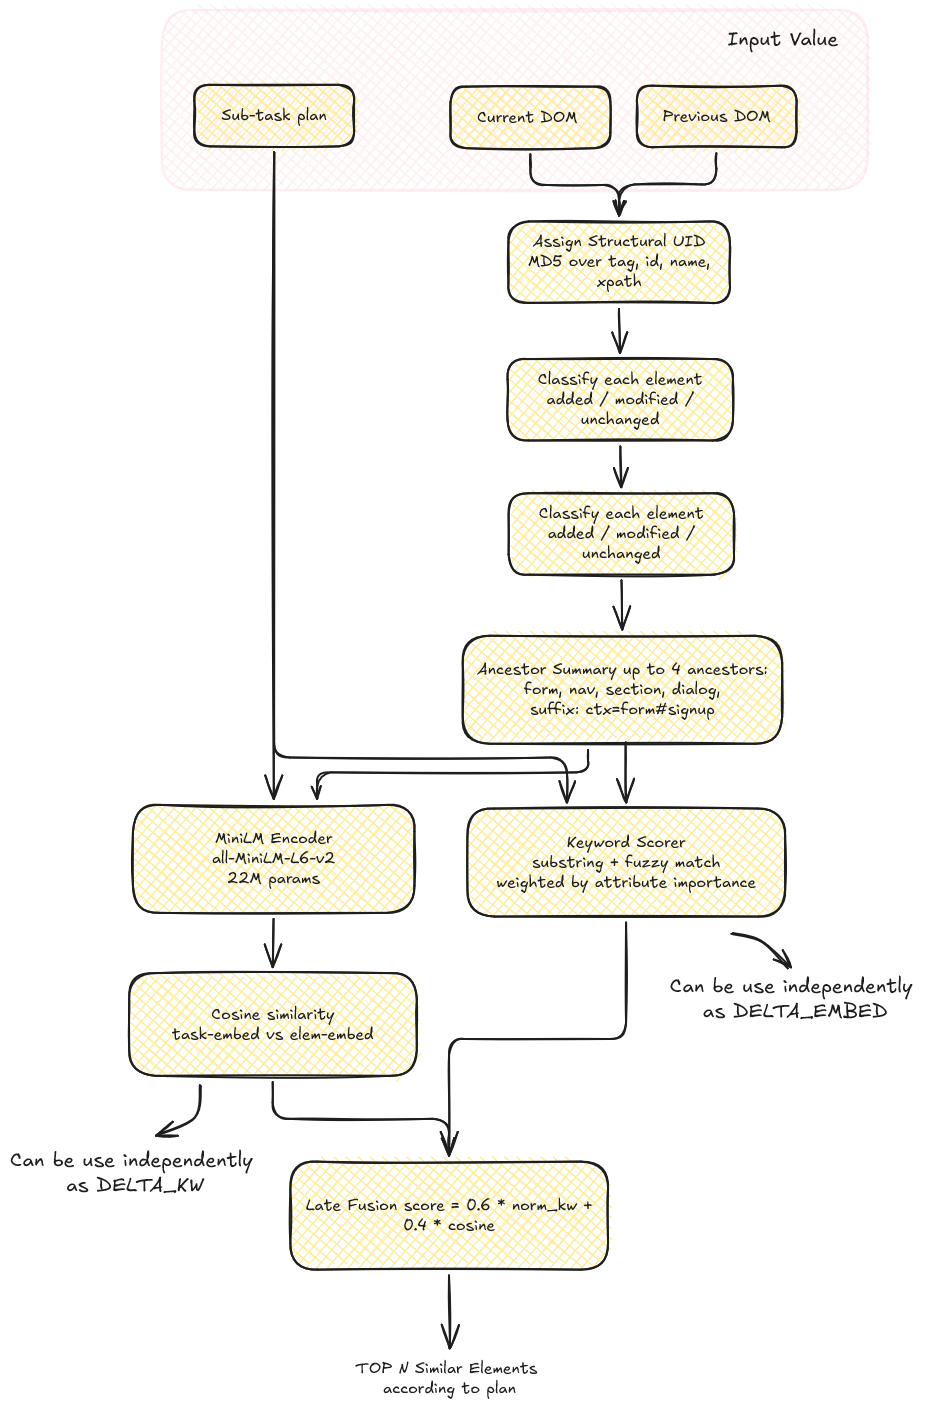
\includegraphics[width=\linewidth,height=0.72\textheight,keepaspectratio]{DOM_DELTA_DIAGRAM.png}
      \end{flushright}
    \end{column}
  \end{columns}
\end{frame}


% --- Slide 16: Novelty 2 ---
% Slide 16: Novelty 2: Policy Hub + Risk-Based HITL
\begin{frame}{Novelty 2: Policy Hub + Risk-Based HITL}
  \footnotesize
  \begin{itemize}
    \item \textbf{PolicyHub:} Contains policies and risky keywords list, which is customizable and can contain complete policy as well.

    \item LLM JSON output extended with \texttt{policy\_risk} (bool), \texttt{risk\_confidence}, \texttt{hitl\_reason}.

    \item \textbf{HITL gate} fires on any one of three OR-combined triggers:
    \begin{enumerate}
      \item[(a)] LLM self-flags \texttt{policy\_risk=true},
      \item[(b)] a risk keyword appears in the action text or \texttt{hitl\_reason},
      \item[(c)] \texttt{risk\_confidence} falls below a configured threshold.
    \end{enumerate}

    \item The gate sits \textbf{before the grounder}, so risky steps further inference can be avoided by the expensive grounder call.

    \item \textbf{Privacy-Aware LLM wrapper} (between Filter and Grounder) runs a regex PII detector (email, phone, Aadhaar, PAN, password) and replaces matches with \texttt{[EMAIL\_MASKED]} style placeholders.
    \item A short privacy directive is injected into the grounder prompt so masked tokens are treated as opaque.
  \end{itemize}
\end{frame}


% --- Slide 17: Architecture ---
% Slide 17: Architecture
\begin{frame}{Architecture}
  \begin{columns}[T,onlytextwidth]
    \begin{column}{0.48\textwidth}
      \begin{description}
        \item[Action Generation (LMM):] Given the current screenshot + task + history to model which returns a textual action and risk scores for action.
        \item[Action Grounding:] Map textual description to actual DOM element + operation (click / type / select) by small model and with DOM delta methodology.
        \item[Browser Execution:] Use automation (via Playwright / browser engine) to execute the action. Webpage updates and we get new screenshot + DOM.
      \end{description}
    \end{column}
    \begin{column}{0.50\textwidth}
      \begin{flushright}
        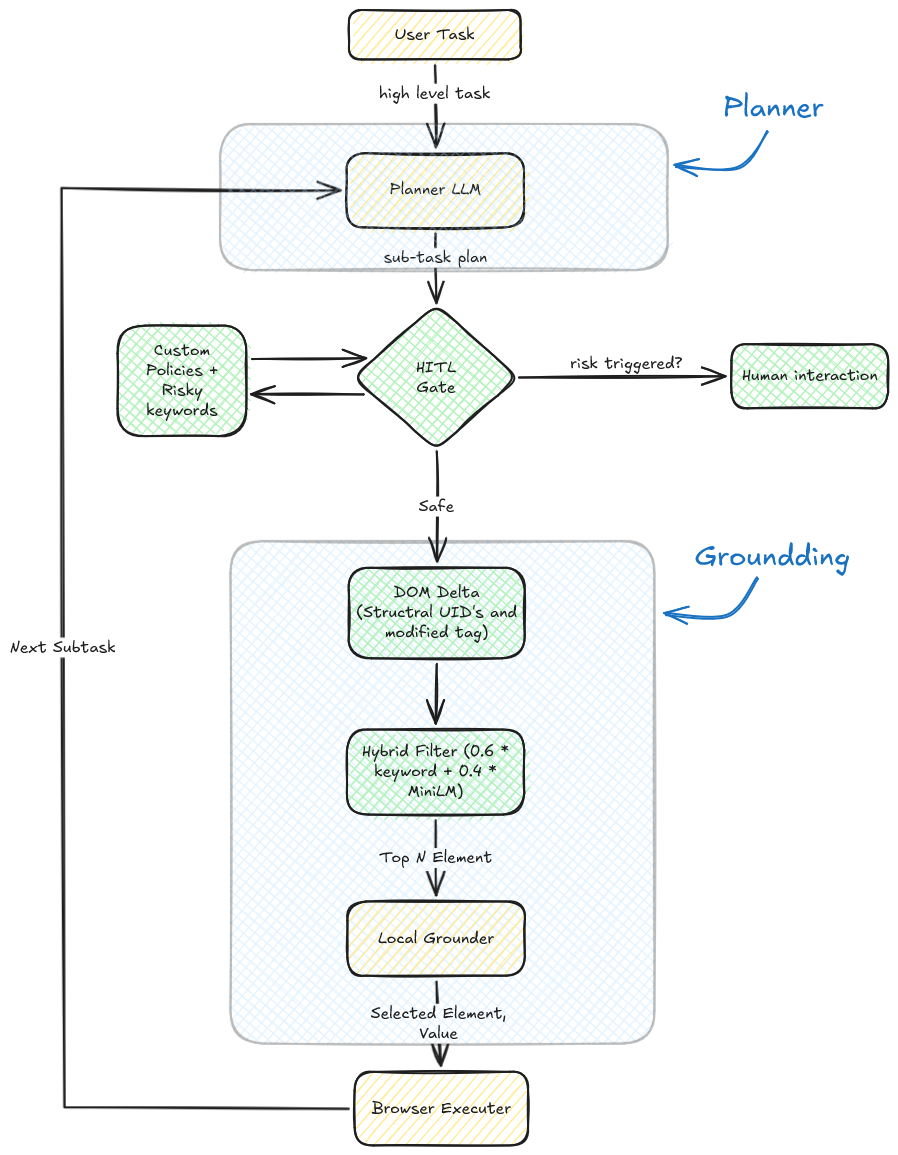
\includegraphics[width=\linewidth,height=0.74\textheight,keepaspectratio]{Architecture.png}
      \end{flushright}
    \end{column}
  \end{columns}
\end{frame}


% --- Slide 18: Improvement ---
% Slide 18: Improvement
\begin{frame}{Improvement}
  \begin{columns}[T]
    \begin{column}{0.48\textwidth}
      \textbf{Prune4Web:}
      \begin{align*}
        a_t &= \pi(s_t, T, \{a_1, a_2, \ldots, a_{t-1}\}) \\
        s_{t+1} &= S(a_t) = \{h_{t+1}, i_{t+1}\}
      \end{align*}
      \textbf{Where:}\\
      $a_t$ = action at time $t$\\
      $s$ = site specific input (html + image)\\
      $\pi$ = Multimodal LLM\\
      $T$ = user defined task
    \end{column}

    \begin{column}{0.48\textwidth}
      \textbf{Our's:}
      \begin{align*}
        A_t &= \pi(s_t, T, \{a_1, a_2, \ldots, a_{t-1}\}, p_t) \\
        s_{t+1} &= S(a_t) = \{h_{t+1}, i_{t+1}\}
      \end{align*}
      \textbf{Where:}\\
      $a_t$ = action at time $t$\\
      $s$ = site specific input (html + image)\\
      $\pi$ = Multimodal LLM\\
      $T$ = user defined task\\
      $p_t$ = Policy rules\\
      $A_t \in (a_t, c, r, h_r)$\\
      $c$ = confidence, $c \in [0,100]$\\
      $r \in \{0,1\}$\\
      $h_r$ = \texttt{hitl\_reason}
    \end{column}
  \end{columns}
\end{frame}


% --- Slide 19: Improvement Algorithm ---
% Slide 19: Improvement - Algorithm
\begin{frame}{Improvement -- Algorithm}
  \begin{block}{Algorithm: Policy-Aware Action Loop}
    \ttfamily\small
    \begin{tabbing}
      \hspace{0.5cm}\=\hspace{0.5cm}\=\hspace{0.5cm}\=\kill
      $A_t = \pi(s_t, T, \{a_1, a_2, \ldots, a_{t-1}\}, p_t)$ \\[2pt]
      $a_t, c, r, h_r = A_t$ \\[2pt]
      matched = compare action plan and policy keywords \\[4pt]
      \textbf{if} $(r > 0$ \textbf{or} matched \textbf{or} $c < \text{confidence})$ \{ \\
      \> $r = 1$ \hspace{1cm} \# policy\_risk detected \\
      \} \\[4pt]
      \textbf{if} $(r == 1)$ \{ \\
      \> HITL value triggered, wait for human interaction for step \\
      \} \textbf{else} \{ \\
      \> Execute further steps from grounding \\
      \}
    \end{tabbing}
  \end{block}
\end{frame}


% --- Slide 20: Implementation Notes ---
% Slide 20: Implementation Notes
\begin{frame}{Implementation Notes}
  \begin{itemize}
    \item Our architecture inspired from Prune4Web with some deviations.

    \item \textbf{Grounder:} QLoRA-fine-tuned Qwen2.5-0.5B or Qwen3-0.6B loaded in 4-bit nf4; $<$1\,GB VRAM at inference on RTX 4050 (6\,GB).

    \item Fine-tuned on 6,626 Mind2Web examples using the identical grounder prompt as inference --- no train/inference drift.

    \item DOM Delta + Privacy wrapper run entirely on-device.
  \end{itemize}
\end{frame}


% --- Slide 21: Filter-Stage Recall ---
% Slide 21: Experiments: Filter-Stage Recall@20
\begin{frame}{Experiments: Filter-Stage Recall@20}
  \begin{center}
    \scriptsize
    \begin{tabular}{l r r r r r}
      \toprule
      \textbf{Split} & \textbf{Samples} & \textbf{FULL R@20} & \textbf{DELTA\_HYBRID R@20} & \textbf{$\Delta$} & \textbf{Token red.} \\
      \midrule
      test\_task    & 1,257 & 90.30\% & 90.07\% & $-0.23$\,pp & 17.8\% \\
      test\_website & 975   & 89.95\% & 89.85\% & $-0.10$\,pp & 16.4\% \\
      test\_domain  & 3,838 & 86.78\% & 87.98\% & $+1.20$\,pp & 17.5\% \\
      \bottomrule
    \end{tabular}
  \end{center}

  \vskip0.5cm
  DELTA\_HYBRID matches FULL Recall@20 within 0.23\,pp on two splits and \textbf{improves} on the largest split, while reducing grounder input tokens by \textbf{16--18\%}.
\end{frame}


% --- Slide 22: Grounder EA ---
% Slide 22: Experiments: Grounder Element Accuracy
\begin{frame}{Experiments: Grounder Element Accuracy}
  \begin{center}
    \begin{tabular}{l r r l}
      \toprule
      \textbf{Grounder} & \textbf{Params} & \textbf{test\_task EA} & \textbf{Notes} \\
      \midrule
      Qwen2.5VL-3B-Instruct (Prune4Web) & 3.0B & 88.28\% & Vision-language, paper baseline \\
      Qwen2.5-0.5B + QLoRA (ours) & 0.5B & 85.00\% & Text-only, 6$\times$ fewer params \\
      Qwen3-0.6B + QLoRA (ours) & 0.6B & 88.00\% & Text-only, 5$\times$ fewer params, matches paper \\
      \bottomrule
    \end{tabular}
  \end{center}

  \vskip0.5cm
  200-sample \texttt{test\_domain} slice with DOM Delta enabled: Qwen3 reaches \textbf{88.00\% EA}, matching the 3B vision-language baseline within rounding margin while running without a vision encoder.
\end{frame}


% --- Slide 23: HITL Results ---
% Slide 23: Implementation & Initial Result
\begin{frame}{Implementation \& Initial Result}
  {\small *Initial results are computed on 13 live websites (7 required HITL, 6 not required HITL)}

  \vskip0.2cm
  \begin{columns}[T,onlytextwidth]
    \begin{column}{0.56\textwidth}
      \scriptsize
      \setlength{\tabcolsep}{5pt}
      \begin{tabular}{l r}
        \toprule
        \textbf{Metric} & \textbf{Value} \\
        \midrule
        HITL Recall         & 85.71\% \\
        HITL Precision      & 100\%   \\
        HITL Accuracy       & 92.86\% \\
        False Positive Rate & 0\%     \\
        False Negative Rate & 14.29\% \\
        \bottomrule
      \end{tabular}

      \vskip0.25cm
      \footnotesize
      \begin{itemize}
        \item The system is able in triggering HITL.
        \item It avoids unnecessary human interruptions (0 false positives),
        \item but misses some high-risk cases (false negatives),
        \item which we aim to improve via expanded risk keywords and site-level overrides.
      \end{itemize}
    \end{column}
    \begin{column}{0.42\textwidth}
      \begin{flushright}
        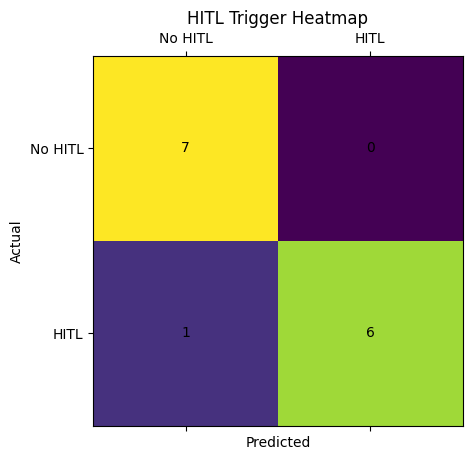
\includegraphics[width=\linewidth,height=0.62\textheight,keepaspectratio]{HITL_Result.png}
      \end{flushright}
    \end{column}
  \end{columns}
\end{frame}


% --- Slide 24: Future Work ---
% Slide 24: Future Work
\begin{frame}{Future Work}
  \begin{itemize}
    \item Future work should focus on gathering data for evaluating PolicyHub and privacy layer on large scale.

    \item Even though Recall@20 of FULL and DELTA HYBRID is $\sim$1\,pp, we observed a stable 5 to 6\,pp Element Accuracy gap between the same QLoRA grounder and the 3B model, even though they differ by only on the same 200 test domain samples.

    \item Experiment should try to reorder top-20 block before grounding and to re-measure EA with both grounders. If the gap closes, candidate-order normalisation should be folded back into the DOM Delta layer. If it does not, the grounder is sensitive to the score-induced ordering itself, which would motivate a small preference-tuning round on ordered candidate blocks.
  \end{itemize}
\end{frame}


% --- Slide 25: Conclusion ---
% Slide 25: Conclusion
\begin{frame}{Conclusion}
  \small
  \begin{itemize}
    \item \textbf{DOM Delta Processing} replaces the stateless full-DOM filter with a structural-UID-tracked delta view. Hybrid keyword + MiniLM scoring gives \textbf{16--18\% token reduction} at matched or improved Recall@20 across 6,070 Mind2Web test samples.

    \item A \textbf{QLoRA-fine-tuned Qwen3-0.6B} local grounder reaches \textbf{88.00\% EA}, matching the Prune4Web 3B Qwen2.5VL-Instruct baseline (88.28\%) within rounding margin while running at 5$\times$ fewer parameters, no vision encoder, $<$1\,GB VRAM on a 6\,GB RTX 4050.

    \item A \textbf{PolicyHub + risk-based HITL gate} with a regex PII detector and a privacy directive injected into the grounder prompt brings privacy-awareness into the action loop, not bolted on after.

    \item \textbf{Net result:} the Prune4Web pipeline becomes cheaper at the filter stage, safer at the grounder stage, and deployable on consumer hardware without sacrificing element accuracy.
  \end{itemize}
\end{frame}


% --- Slides 26-28: References ---
% Slides 26-28: References (manual, fast compile)
\begin{frame}[allowframebreaks]{References}
\footnotesize
\begin{thebibliography}{99}

\bibitem{SeeAct}
Zheng, B., Gou, B., Kil, J., Sun, H., Su, Y. (2024).
\newblock GPT-4V(ision) is a Generalist Web Agent, if Grounded.
\newblock arXiv:2401.01614.

\bibitem{deng2023mind2webgeneralistagentweb}
Deng, X. et al. (2023).
\newblock Mind2Web: Towards a Generalist Agent for the Web.
\newblock arXiv:2306.06070.

\bibitem{lai2024autowebglm}
Lai, H. et al. (2024).
\newblock AutoWebGLM: A Large Language Model-based Web Navigating Agent.
\newblock arXiv:2404.03648.

\bibitem{tarsariya2024agente}
Abuelsaad, T. et al. (2024).
\newblock Agent-E: From Autonomous Web Navigation to Foundational Design Principles in Agentic Systems.
\newblock arXiv:2407.13032.

\bibitem{gur2024webagent}
Gur, I. et al. (2024).
\newblock A Real-World WebAgent with Planning, Long Context Understanding, and Program Synthesis.
\newblock arXiv:2307.12856.

\bibitem{zhang2025largelanguagemodelbrainedgui}
Zhang, C. et al. (2025).
\newblock Large Language Model-Brained GUI Agents: A Survey.
\newblock arXiv:2411.18279.

\bibitem{ning2025surveywebagentsnextgenerationai}
Ning, L. et al. (2025).
\newblock A Survey of WebAgents: Towards Next-Generation AI Agents for Web Automation with Large Foundation Models.
\newblock arXiv:2503.23350.

\bibitem{zhang2025prune4web}
Zhang, J. et al. (2025).
\newblock Prune4Web: DOM Tree Pruning Programming for Web Agent.
\newblock arXiv:2511.21398.

\bibitem{schiepanski2025d2snap}
Schiepanski, T. M., Pi{\"e}l, N. (2025).
\newblock Beyond Pixels: Exploring DOM Downsampling for LLM-Based Web Agents.
\newblock arXiv:2508.04412.

\bibitem{reimers2019sbert}
Reimers, N., Gurevych, I. (2019).
\newblock Sentence-BERT: Sentence Embeddings using Siamese BERT-Networks.
\newblock arXiv:1908.10084.

\bibitem{wang2020minilm}
Wang, W. et al. (2020).
\newblock MiniLM: Deep Self-Attention Distillation for Task-Agnostic Compression of Pre-Trained Transformers.
\newblock arXiv:2002.10957.

\bibitem{dettmers2023qlora}
Dettmers, T., Pagnoni, A., Holtzman, A., Zettlemoyer, L. (2023).
\newblock QLoRA: Efficient Finetuning of Quantized LLMs.
\newblock arXiv:2305.14314.

\bibitem{tang2025surveymllmbasedguiagents}
Tang, F. et al. (2025).
\newblock A Survey on (M)LLM-Based GUI Agents.
\newblock arXiv:2504.13865.

\bibitem{wang2025guiagentsfoundationmodels}
Wang, S. et al. (2025).
\newblock GUI Agents with Foundation Models: A Comprehensive Survey.
\newblock arXiv:2411.04890.

\bibitem{FewShotLearning:verma2024adaptagentadaptingmultimodalweb}
Verma, G. et al. (2024).
\newblock AdaptAgent: Adapting Multimodal Web Agents with Few-Shot Learning from Human Demonstrations.
\newblock arXiv:2411.13451.

\bibitem{zhang2025litewebagentopensourcesuitevlmbased}
Zhang, D. et al. (2025).
\newblock LiteWebAgent: The Open-Source Suite for VLM-Based Web-Agent Applications.
\newblock arXiv:2503.02950.

\bibitem{iong2024openwebagent}
Iong, I. L. et al. (2024).
\newblock Openwebagent: An open toolkit to enable web agents on large language models.
\newblock ACL System Demonstrations.

\bibitem{Browsinglikehuman:luo2025browsing}
Luo, H. et al. (2025).
\newblock Browsing like human: A multimodal web agent with experiential fast-and-slow thinking.
\newblock ACL Long Papers.

\end{thebibliography}
\end{frame}


% --- Slide 29: Thanks ---
% Slide 29: Thanks
{
\setbeamertemplate{footline}{}
\begin{frame}[plain]
  \vfill
  \centering
  {\Huge\bfseries\color{primaryNavy} Thanks!}

  \vskip1cm
  {\Large Do have any questions?}
  \vfill
\end{frame}
}


\end{document}
